\section{Bài toán dẫn đến bài toán quy hoạch tuyến tính}
Trong thực tế, có rất nhiều vấn đề kinh tế, kỹ thuật đòi hỏi chúng ta phải tìm ra phương án hoạt động tốt nhất (tối ưu nhất) trong điều kiện các nguồn lực bị giới hạn. Việc chuyển ngữ các vấn đề này thành các phương trình, bất phương trình toán học được gọi là quá trình thiết lập mô hình. 

Dưới đây là một ví dụ điển hình về việc xây dựng mô hình toán học cho bài toán lập kế hoạch sản xuất.

\begin{exampleblock}{Ví dụ: Bài toán sản xuất tối ưu}
Một Công ty sản xuất bánh trung thu cần sản xuất 3 loại sản phẩm bánh (L1, L2, L3) từ 3 loại nguyên liệu chính khác nhau là Đường, Bột và Sữa. 

Giả sử tất cả sản phẩm sản xuất ra đều được tiêu thụ hết. Các thông số về định mức tiêu hao nguyên liệu cho 1 đơn vị sản phẩm, tổng khối lượng nguyên liệu dự trữ và giá bán của từng loại sản phẩm được cho trong bảng sau:

\begin{table}[htbp]
    \centering
    \renewcommand{\arraystretch}{1.2}
    \begin{tabular}{|l|c|c|c|c|}
        \hline
        \multirow{2}{*}{\textbf{Loại nguyên liệu}} & \multirow{2}{*}{\textbf{\shortstack{Khối lượng \\ dự trữ (g)}}} & \multicolumn{3}{c|}{\textbf{Định mức cho 1 đv sản phẩm (g)}} \\
        \cline{3-5}
        & & \textbf{L1} & \textbf{L2} & \textbf{L3} \\
        \hline
        Đường & 10.000 & 10 & 20 & 20 \\
        \hline
        Bột   & 50.000 & 20 & 30 & 30 \\
        \hline
        Sữa   & 30.000 & 20 & 30 & 40 \\
        \hline
        \textbf{Giá bán 1 đv sp (\$)} & \textbf{-} & \textbf{2} & \textbf{3} & \textbf{4} \\
        \hline
    \end{tabular}
    \caption{Thông số bài toán sản xuất bánh trung thu}
\end{table}

\textbf{Yêu cầu:} Hãy lập kế hoạch sản xuất tối ưu cho Công ty (sản xuất như thế nào để tổng doanh thu đạt được là cao nhất)?

\textbf{Thiết lập mô hình toán học:}
Gọi $x_j$ ($j = 1, 2, 3$) lần lượt là số lượng sản phẩm bánh loại $L_j$ cần sản xuất. 
Vì số lượng sản phẩm không thể mang giá trị âm, ta có điều kiện: $x_1, x_2, x_3 \ge 0$.

Tổng khối lượng nguyên liệu các loại dùng để sản xuất 3 sản phẩm không được vượt quá số lượng dự trữ:
\begin{itemize}
    \item Lượng đường sử dụng: $10x_1 + 20x_2 + 20x_3 \le 10000$.
    \item Lượng bột sử dụng: $20x_1 + 30x_2 + 30x_3 \le 50000$.
    \item Lượng sữa sử dụng: $20x_1 + 30x_2 + 40x_3 \le 30000$.
\end{itemize}

Tổng doanh thu Công ty thu được khi bán hết sản phẩm là hàm mục tiêu cần đạt giá trị lớn nhất:
\begin{equation*}
    Z = 2x_1 + 3x_2 + 4x_3 \rightarrow \max
\end{equation*}

Tóm lại, mô hình toán học của bài toán sản xuất tối ưu trên được viết gọn lại dưới dạng hệ như sau:
\[
\begin{aligned}
    Z &= 2x_1 + 3x_2 + 4x_3 \rightarrow \max \\
    \text{s.t.} \quad 10x_1 + 20x_2 + 20x_3 &\le 10000 \\
    20x_1 + 30x_2 + 30x_3 &\le 50000 \\
    20x_1 + 30x_2 + 40x_3 &\le 30000 \\
    x_1, x_2, x_3 &\ge 0
\end{aligned}
\]

\end{exampleblock}

\begin{remarkblock}{Một số dạng bài toán khác trong thực tế}
Bên cạnh bài toán lập kế hoạch sản xuất, mô hình quy hoạch tuyến tính còn được ứng dụng rộng rãi để giải quyết nhiều lớp bài toán thực tế khác như:
\begin{itemize}
    \item \textbf{Bài toán xác định khẩu phần ăn tối ưu:} Tìm lượng thức ăn cần mua sao cho thỏa mãn đủ các chất dinh dưỡng cần thiết (đạm, béo, vitamin...) với chi phí đi chợ là nhỏ nhất.
    \item \textbf{Bài toán pha trộn:} Pha trộn các nguyên liệu đầu vào với tỷ lệ nào để tạo ra sản phẩm đạt tiêu chuẩn kỹ thuật với giá thành rẻ nhất.
    \item \textbf{Bài toán bổ nhiệm/phân công:} Phân công nhân sự vào các vị trí công việc khác nhau sao cho tổng hiệu suất làm việc đạt mức cực đại.
\end{itemize}
\end{remarkblock}


% =================================================================================
% =================================- PP Hình học -=================================
% =================================================================================

\section{Phân loại các loại Phương án trong QHTT}
Trong Quy hoạch tuyến tính, việc tìm ra lời giải giống như một quá trình "sàng lọc" qua nhiều cấp độ. Đi từ tập hợp tất cả các con số có thể có, ta lọc ra những con số hợp lệ, sau đó tìm những điểm đáng chú ý nhất, và cuối cùng chọn ra người chiến thắng. 

Dưới đây là 3 cấp độ phân loại phương án cốt lõi của bài toán QHTT:

\subsubsection{1. Phương án (PA - Phương án chấp nhận được)}
\begin{definition}[Phương án]
Một vector $n$ chiều $x = (x_1, x_2, \dots, x_n) \in \mathbb{R}^n$ thỏa mãn \textbf{toàn bộ hệ ràng buộc chính} và \textbf{ràng buộc dấu} được gọi là một phương án chấp nhận được (hay gọi tắt là Phương án).
\end{definition}

\textbf{Ký hiệu toán học:}
\begin{itemize}
    \item Tập hợp tất cả các phương án hợp lệ của bài toán được gọi là \textbf{Tập phương án} (hay miền ràng buộc), ký hiệu là $\Omega$. 
    \item Nếu $x \in \Omega$, ta nói $x$ là một phương án.
\end{itemize}

\textbf{Giải thích trực quan:} 
Hãy tưởng tượng bạn có 100.000 VNĐ để đi chợ mua thịt và rau. Bất kỳ sự kết hợp nào (ví dụ: mua 2 lạng thịt, 1 mớ rau) mà tổng tiền thanh toán $\le 100.000$ VNĐ và số lượng mua không bị âm ($\ge 0$) thì đều được coi là một "Phương án". Tập hợp $\Omega$ chính là cái giỏ chứa \textit{tất cả} các cách đi chợ hợp lệ đó.

\subsubsection{2. Phương án cơ bản (PACB)}
Trong số hàng ngàn phương án hợp lệ, có những phương án nằm ở vị trí đặc biệt (các "góc" hoặc "đỉnh" của miền ràng buộc). Đó chính là các phương án cơ bản.

\begin{definition}[Phương án cơ bản]
Một phương án được gọi là \textbf{Phương án cơ bản (PACB)} nếu nó thỏa mãn ít nhất $n$ ràng buộc với dấu đẳng thức ($=$).
\end{definition}

\textbf{Phân loại chi tiết PACB:}
\begin{itemize}
    \item \textbf{PACB không suy biến:} Là PACB thỏa mãn \textit{đúng} $n$ ràng buộc với dấu đẳng thức ($=$). Đây là trường hợp lý tưởng nhất, đại diện cho một đỉnh chuẩn xác trên đồ thị.
    \item \textbf{PACB suy biến:} Xảy ra khi có nhiều hơn $n$ ràng buộc vô tình cùng giao nhau tại một điểm.
\end{itemize}

\textbf{Giải thích trực quan:} 
Quay lại ví dụ đi chợ, nếu bạn mua một lượng thịt và rau sao cho \textit{tiêu sạch sành sanh} đúng 100.000 VNĐ (dấu $=$ xảy ra ở ràng buộc túi tiền), bạn đang chạm đến "giới hạn" khả năng của mình. Trong toán học tối ưu, người ta chứng minh được rằng: \textit{Nếu bài toán có lời giải tốt nhất, lời giải đó chắc chắn nằm ở một trong các Phương án cơ bản (các đỉnh giới hạn) này}. Đó là lý do thuật toán Đơn hình chỉ tập trung nhảy từ PACB này sang PACB khác chứ không tìm kiếm mò mẫm ở giữa miền.

\subsubsection{3. Phương án tối ưu (PATƯ)}
Đây là đích đến cuối cùng của mọi bài toán QHTT.

\begin{definition}[Phương án tối ưu]
Một phương án $x^*$ được gọi là Phương án tối ưu (PATƯ) nếu nó vừa là phương án hợp lệ ($x^* \in \Omega$), vừa làm cho hàm mục tiêu $Z(x)$ đạt giá trị lớn nhất (Max) hoặc nhỏ nhất (Min) tùy theo yêu cầu bài toán.
\end{definition}

\textbf{Ký hiệu toán học:}
\begin{itemize}
    \item $x^*$: Vector phương án tối ưu (Lời giải của bài toán).
    \item $Z_{max}$ hoặc $Z_{min}$: Giá trị tối ưu của hàm mục tiêu.
\end{itemize}

\textbf{Giải thích trực quan:} 
Trong tất cả các cách tiêu tiền hợp lệ (Tập PA) và các cách tiêu sạch tiền (Các PACB), "Phương án tối ưu" là cách mua sắm mang lại cho bạn bữa ăn có tổng lượng dinh dưỡng (Hàm mục tiêu $Z$) cao nhất.

\vspace{0.5cm}
\begin{center}
\textbf{TÓM TẮT MỐI QUAN HỆ (BỨC TRANH TỔNG THỂ)} \\
\textit{Quá trình tìm lời giải bài toán QHTT tuân theo sơ đồ bao hàm sau:} \\
\vspace{0.2cm}
$\mathbf{PATU \subset PACB \subset PA \subset \mathbb{R}^n}$ \\
\textit{(Lời giải tối ưu luôn nằm trong nhóm các phương án cơ bản; Phương án cơ bản là trường hợp đặc biệt của phương án hợp lệ; và phương án hợp lệ được lấy từ không gian số thực $n$ chiều).}
\end{center}

\section{Các dạng đặc biệt và Biến đổi mô hình}

\begin{figure}[htbp]
    \centering
    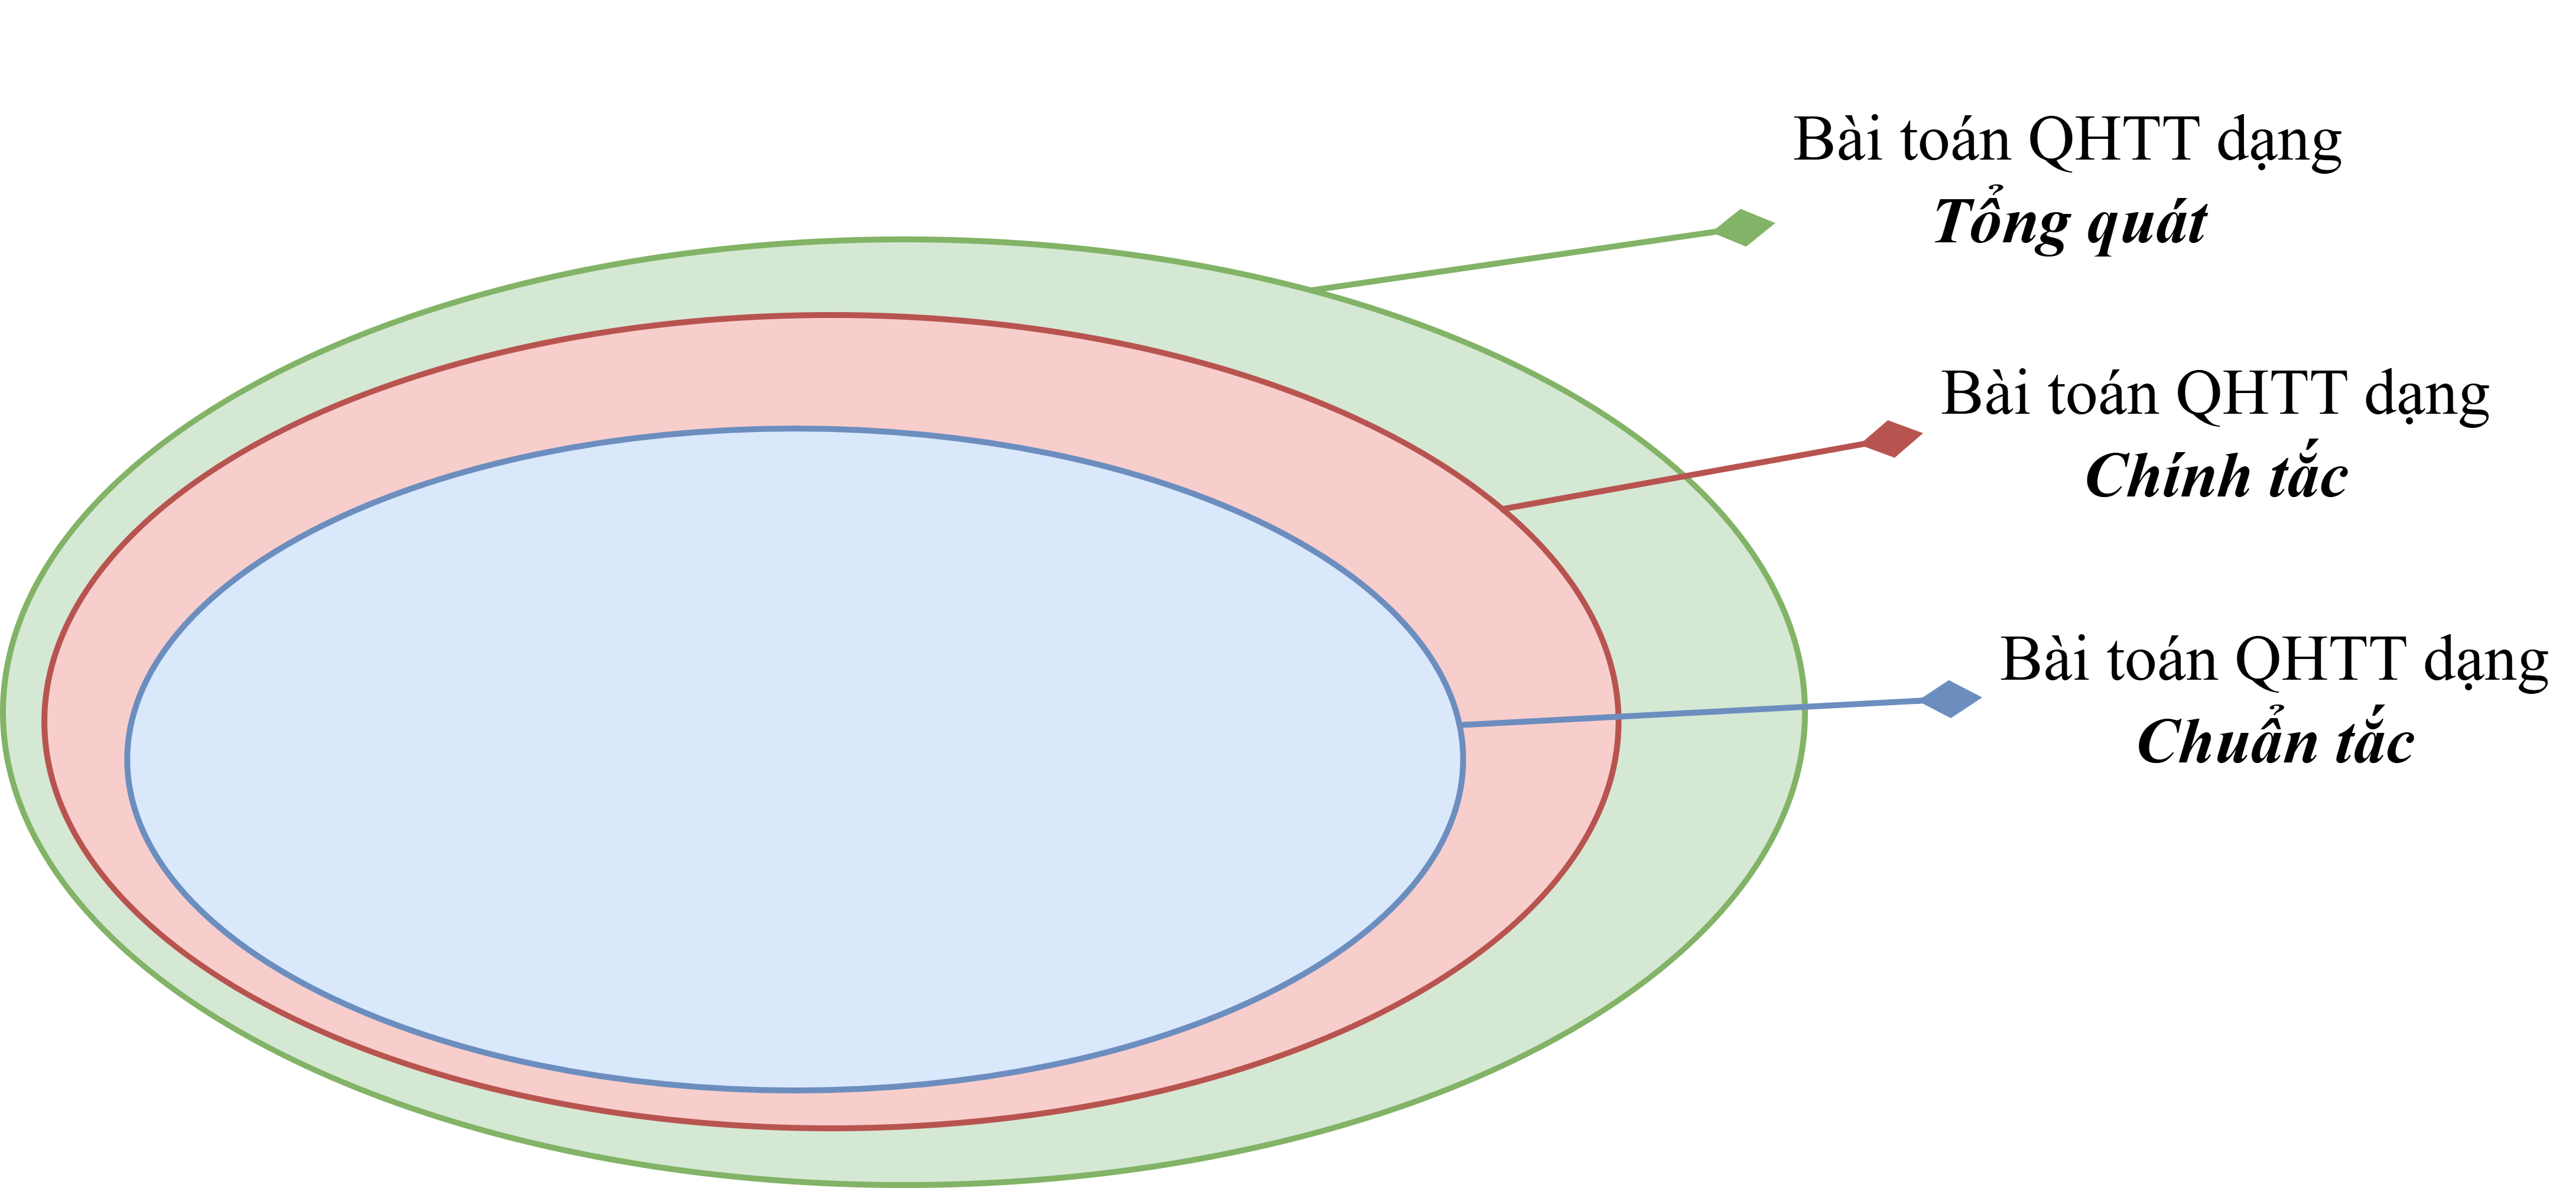
\includegraphics[width=1\linewidth]{images/Graphic.drawio.png}
    \caption{Sơ đồ phân loại 3 dạng bài toán QHTT}
    \label{fig:phanloai_qhtt}
\end{figure}

\subsection{Bài toán QHTT tổng quát}
Từ các bài toán thực tế, ta có thể tổng quát hóa mô hình toán học của một bài toán Quy hoạch tuyến tính (QHTT) dưới dạng sau:

\textbf{Hàm mục tiêu:}
\begin{formula}
    Z = \sum_{j=1}^{n} c_j x_j \rightarrow \max (\text{hoặc } \min)
\end{formula}

\textbf{Hệ ràng buộc chính:}
\begin{formula}
    \sum_{j=1}^{n} a_{ij} x_j 
    \begin{bmatrix} 
        \ge \\ 
        \le \\ 
        = 
    \end{bmatrix} 
    b_i, \quad (i = \overline{1,m})
\end{formula}

\textbf{Ràng buộc dấu:}
\begin{formula}
    x_j 
    \begin{bmatrix} 
        \ge 0 \\ 
        \le 0 \\ 
        \text{tùy ý} 
    \end{bmatrix}, \quad (j = \overline{1,n})
\end{formula}

Trong đó:
\begin{itemize}
    \item $x_j$: Các biến quyết định (ẩn số cần tìm).
    \item $c_j$: Các hệ số của hàm mục tiêu.
    \item $a_{ij}$: Các hệ số công nghệ (nằm ở dòng $i$, cột $j$).
    \item $b_i$: Giá trị giới hạn vế phải của các ràng buộc.
\end{itemize}

\subsection{Tính chất cốt lõi của bài toán QHTT}
Dựa trên các khái niệm về phương án, một bài toán QHTT luôn tuân theo các tính chất toán học sau:
\begin{itemize}
    \item Nếu bài toán tìm Max (hoặc Min) có tập phương án không rỗng và hàm mục tiêu bị chặn trên (hoặc chặn dưới), thì bài toán chắc chắn có phương án tối ưu.
    \item Nếu bài toán QHTT có nhiều hơn một PATƯ thì nó sẽ có vô số PATƯ. 
    \item \textbf{Cụ thể:} Nếu $x^0$ và $x^1$ là hai phương án tối ưu phân biệt, thì mọi bao lồi (tổ hợp lồi) của chúng có dạng:
    \begin{equation*}
        x = \alpha x^0 + (1-\alpha)x^1, \quad \text{với } \alpha \in
    \end{equation*}
    cũng là một phương án tối ưu của bài toán này.
\end{itemize}


Để thuận lợi cho việc áp dụng các thuật toán giải quyết trên máy tính, từ bài toán tổng quát, người ta phân loại và biến đổi mô hình về 3 dạng đặc biệt sau:

\subsection{Bài toán QHTT dạng chính tắc}
Bài toán QHTT dạng chính tắc là bài toán có tất cả các ràng buộc chính ở dạng đẳng thức ($=$) và mọi ràng buộc dấu đều không âm ($x_j \ge 0$).

Mô hình toán học có dạng:
\begin{formula}
    \begin{aligned}
    Z = \sum_{j=1}^{n} c_j x_j \rightarrow \max (\text{hoặc } \min) \\
    \sum_{j=1}^{n} a_{ij} x_j = b_i, \quad (i = \overline{1,m}) \\
    x_j \ge 0, \quad (j = \overline{1,n})
    \end{aligned}
\end{formula}


\textbf{Ma trận điều kiện:} Ma trận $A = (a_{ij})$ chứa các hệ số của hệ ràng buộc chính được gọi là ma trận điều kiện. Cột thứ $j$ của ma trận $A$ (ký hiệu $A_j$) được gọi là vector điều kiện của biến $x_j$.

\subsection{Bài toán QHTT dạng chuẩn}
Bài toán QHTT được gọi là có dạng chuẩn nếu nó đã ở dạng chính tắc, vế phải của các ràng buộc không âm ($b_i \ge 0$) và \textbf{mỗi ràng buộc chính phải có một biến cơ sở}.

\textit{Biến cơ sở} ứng với một phương trình ràng buộc là biến có hệ số bằng 1 ở phương trình đó và có hệ số bằng 0 ở tất cả các phương trình còn lại.

Mô hình dạng chuẩn được viết phân tách như sau:

\begin{formula}
\begin{alignedat}{4}
    Z = & \sum_{j=1}^{n} c_j x_j & \rightarrow \max (\text{hoặc } \min) \\
    \text{s.t.} \quad & x_1 + a_{1, m+1}x_{m+1} + \dots + a_{1n}x_n & = b_1 \\
    & x_2 + a_{2, m+1}x_{m+1} + \dots + a_{2n}x_n & = b_2 \\
    & \dots \\
    & x_m + a_{m, m+1}x_{m+1} + \dots + a_{mn}x_n & = b_m \\
    & \rlap{$x_j \ge 0, \quad b_i \ge 0$}
\end{alignedat}    
\end{formula}

Trong mô hình trên, các biến $x_1, x_2, \dots, x_m$ đóng vai trò là các biến cơ sở, trong khi $x_{m+1}, \dots, x_n$ là các biến không cơ sở.

\subsection{Kỹ thuật biến đổi mô hình QHTT}
Để áp dụng được thuật toán Đơn hình, mọi bài toán QHTT đều phải được đưa về dạng Chuẩn tắc. Dưới đây là các phép biến đổi cơ bản:

\textbf{1. Biến đổi Ràng buộc chính (Đưa về dấu $=$):}
\begin{itemize}
    \item Nếu ràng buộc thứ $i$ có dấu "$\le$": Ta \textbf{cộng thêm} một \textit{biến phụ} $x_{n+i} \ge 0$ vào vế trái.
    \item Nếu ràng buộc thứ $i$ có dấu "$\ge$": Ta \textbf{trừ đi} một \textit{biến phụ} $x_{n+i} \ge 0$ ở vế trái.
    \item Nếu phương trình thiếu biến cơ sở: Ta \textbf{cộng thêm} một \textit{biến giả} vào vế trái (Kèm theo việc thêm hệ số phạt $\pm M$ trên hàm mục tiêu).
\end{itemize}

\textbf{2. Biến đổi Ràng buộc dấu (Đưa về $\ge 0$):}
\begin{itemize}
    \item Nếu biến $x_j \le 0$: Đặt biến mới $x'_j = -x_j$, khi đó $x'_j \ge 0$. Thay thế $-x'_j$ vào mọi vị trí của $x_j$ trong bài toán.
    \item Nếu biến $x_j$ \textbf{tùy ý} (không ràng buộc dấu): Đặt $x_j = x_j^+ - x_j^-$, với điều kiện $x_j^+, x_j^- \ge 0$.
\end{itemize}


\vspace{0.5cm}
\begin{figure}[H]
    \centering
    \resizebox{\textwidth}{!}{
    \begin{tikzpicture}[
        node distance=2.5cm, % Thu hẹp khoảng cách giữa các hộp một chút
        box/.style={rectangle, rounded corners=8pt, thick, align=left, inner sep=8pt, drop shadow={opacity=0.1}},
        arrow/.style={->, >=stealth, line width=1.5pt}
    ]

    % ==========================================
    % KHỐI 1: TỔNG QUÁT
    % ==========================================
    \node[box, fill=blue!5, draw=blue!80!black] (tongquat) {
        \renewcommand{\arraystretch}{1.6}
        % Chỉnh độ rộng cột nhỏ lại để không bị tràn lề
        \begin{tabular}{p{7cm} | p{6.5cm}}
            \textbf{\Large 1. Dạng Tổng Quát} & \textbf{\Large Mô hình Toán học} \\[0.1cm]
            $\bullet$ \textbf{Hàm mục tiêu:} $Z \rightarrow \max$ hoặc $\min$ & 
            $\displaystyle Z = \sum_{j=1}^n c_j x_j \rightarrow \max (\min)$ \\
            $\bullet$ \textbf{Ràng buộc chính:} Có thể chứa $\le, \ge$ hoặc $=$ & 
            % Dàn phẳng các dấu để không bị giãn chiều cao
            $\displaystyle \sum_{j=1}^n a_{ij} x_j \in \{\le, \ge, =\} \, b_i$ \\
            $\bullet$ \textbf{Ràng buộc dấu:} $x_j \ge 0, \le 0$ hoặc tùy ý & 
            $\displaystyle x_j \in \{\ge 0, \le 0, \text{tùy ý}\}$
        \end{tabular}
    };

    % ==========================================
    % KHỐI 2: CHÍNH TẮC
    % ==========================================
    \node[box, fill=green!5, draw=green!60!black, below=2.5cm of tongquat] (chinhtac) {
        \renewcommand{\arraystretch}{1.6}
        \begin{tabular}{p{7cm} | p{6.5cm}}
            \textbf{\Large 2. Dạng Chính Tắc} & \textbf{\Large Mô hình Toán học} \\[0.1cm]
            $\bullet$ \textbf{Hàm mục tiêu:} $Z \rightarrow \max$ hoặc $\min$ & 
            $\displaystyle Z = \sum_{j=1}^n c_j x_j \rightarrow \max (\min)$ \\
            $\bullet$ \textbf{Ràng buộc chính:} \textcolor{red}{\textbf{Bắt buộc là dấu $=$}} & 
            $\displaystyle \sum_{j=1}^n a_{ij} x_j \;\textcolor{red}{=}\; b_i$ \\
            $\bullet$ \textbf{Ràng buộc dấu:} \textcolor{red}{\textbf{Mọi biến $x_j \ge 0$}} & 
            $\displaystyle x_j \;\textcolor{red}{\ge 0}$
        \end{tabular}
    };

    % ==========================================
    % KHỐI 3: CHUẨN TẮC
    % ==========================================
    \node[box, fill=orange!5, draw=orange!80!black, below=2.5cm of chinhtac] (chuantac) {
        \renewcommand{\arraystretch}{1.6}
        \begin{tabular}{p{7cm} | p{6.5cm}}
            \textbf{\Large 3. Dạng Chuẩn Tắc} & \textbf{\Large Mô hình Toán học} \\[0.1cm]
            $\bullet$ \textbf{Hàm mục tiêu:} $Z \rightarrow \max$ hoặc $\min$ & 
            $\displaystyle Z = \sum_{j=1}^n c_j x_j \rightarrow \max (\min)$ \\
            $\bullet$ \textbf{Ràng buộc \& Vế phải:} Dấu $=$ và \textcolor{red}{\textbf{$b_i \ge 0$}} & 
            $\displaystyle \sum_{j=1}^n a_{ij} x_j = b_i \quad (\textcolor{red}{b_i \ge 0})$ \\
            $\bullet$ \textbf{Cơ sở:} \textcolor{red}{\textbf{Đủ $m$ biến cơ sở}} (Ma trận $I_m$) & 
            $\displaystyle \textcolor{red}{x_i} + \sum_{k=m+1}^n a_{ik} x_k = b_i$ \\
            $\bullet$ \textbf{Ràng buộc dấu:} Mọi biến $x_j \ge 0$ & 
            $\displaystyle x_j \ge 0$
        \end{tabular}
    };

    % ==========================================
    % MŨI TÊN VÀ TEXT GIẢI THÍCH
    % ==========================================
    
    % Từ Tổng quát -> Chính tắc
    \draw[arrow, blue!80!black] (tongquat.south) -- (chinhtac.north) 
        node[midway, fill=white, draw=blue!80!black, thick, rounded corners, align=center, inner sep=6pt, drop shadow={opacity=0.1}] {
            \textbf{\textcolor{blue!80!black}{Bước 1: Khử bất phương trình \& Dấu âm}}\\
            $\le$ thì \textbf{cộng} biến phụ \quad $\Big|$ \quad $\ge$ thì \textbf{trừ} biến phụ \\
            $x_j \le 0 \Rightarrow$ Đặt $x'_j = -x_j$ \quad $\Big|$ \quad $x_j$ tùy ý $\Rightarrow$ Đặt $x_j = x'_j - x''_j$
        };

    % Từ Chính tắc -> Chuẩn tắc
    \draw[arrow, green!60!black] (chinhtac.south) -- (chuantac.north) 
        node[midway, fill=white, draw=green!60!black, thick, rounded corners, align=center, inner sep=6pt, drop shadow={opacity=0.1}] {
            \textbf{\textcolor{green!60!black}{Bước 2: Chuẩn bị cơ sở cho thuật toán}}\\
            $b_i < 0 \Rightarrow$ Nhân cả 2 vế phương trình với $(-1)$ \\
            Thiếu biến cơ sở $\Rightarrow$ Cộng \textbf{biến giả} (Kèm theo thêm $\pm M$ vào $Z$)
        };

    \end{tikzpicture}
    }
    \caption{Sơ đồ đối chiếu lý thuyết và ký hiệu toán học qua các dạng bài toán}
    \label{fig:flowchart_forms}
\end{figure}

\subsection{Bài toán QHTT tương đương}
Trong nhiều trường hợp tính toán, việc chuyển đổi qua lại giữa bài toán tìm lớn nhất (Max) và nhỏ nhất (Min) là cần thiết. Hai bài toán QHTT được gọi là tương đương với nhau khi chúng có chung tập phương án và phương án tối ưu.

Giả sử ta có bài toán gốc tìm Max:
\begin{equation*}
    (P): \quad Z = \sum_{j=1}^{n} c_j x_j \rightarrow \max
\end{equation*}

Thì bài toán tương đương của nó sẽ là tìm Min của hàm đối:
\begin{equation*}
    (P'): \quad Z' = -Z = \sum_{j=1}^{n} (-c_j) x_j \rightarrow \min
\end{equation*}
Điều này có nghĩa là khi giải bài toán, thay vì tìm Max của hàm $Z$, ta có thể tìm Min của hàm $-Z$.

\section{Thuật toán Đơn hình mở rộng}


